\chapter[Problema 02]{Problema 02}

\section{Mensagens Utilizando Ping}

O ping é uma ferramenta útil para testar conectividade da rede entre equipamentos, ele utiliza o protocolo ICMP para enviar e receber mensagens. Dois tipos de mensagens são utilizadas: 

\begin{itemize}
	\item O tipo 8 que corresponde a um comando "ECHO request", emitido pela máquina fonte; 
	\item O tipo 0 que corresponde a um comando "ECHO reply", emitido pelo maquina alcançada; 
\end{itemize}

Para a captura de pacotes foi procedida no Sistema operacional Linux Mint 17.2.0 - amd64 Linux 3.16.0 - 38 GNU/Linux.

A ferramenta de captura utilizada foi Wireshark, no qual foi utilizado o comando a seguir para efetuar a instalação.

\emph{sudo apt-get -y install wireshark}

Após efetuar a instalação, o Wirehark foi iniciado e configurado para analisar os pacotes da interface eth0.

Para efetuar a análise dos pacotes, foi executado o comando ping www.locaweb.com.br e interrompido após o 5 pacote ser enviado. A imagem a seguir apresenta o resultado no terminal.

  \begin{figure}[h]
    \centering

    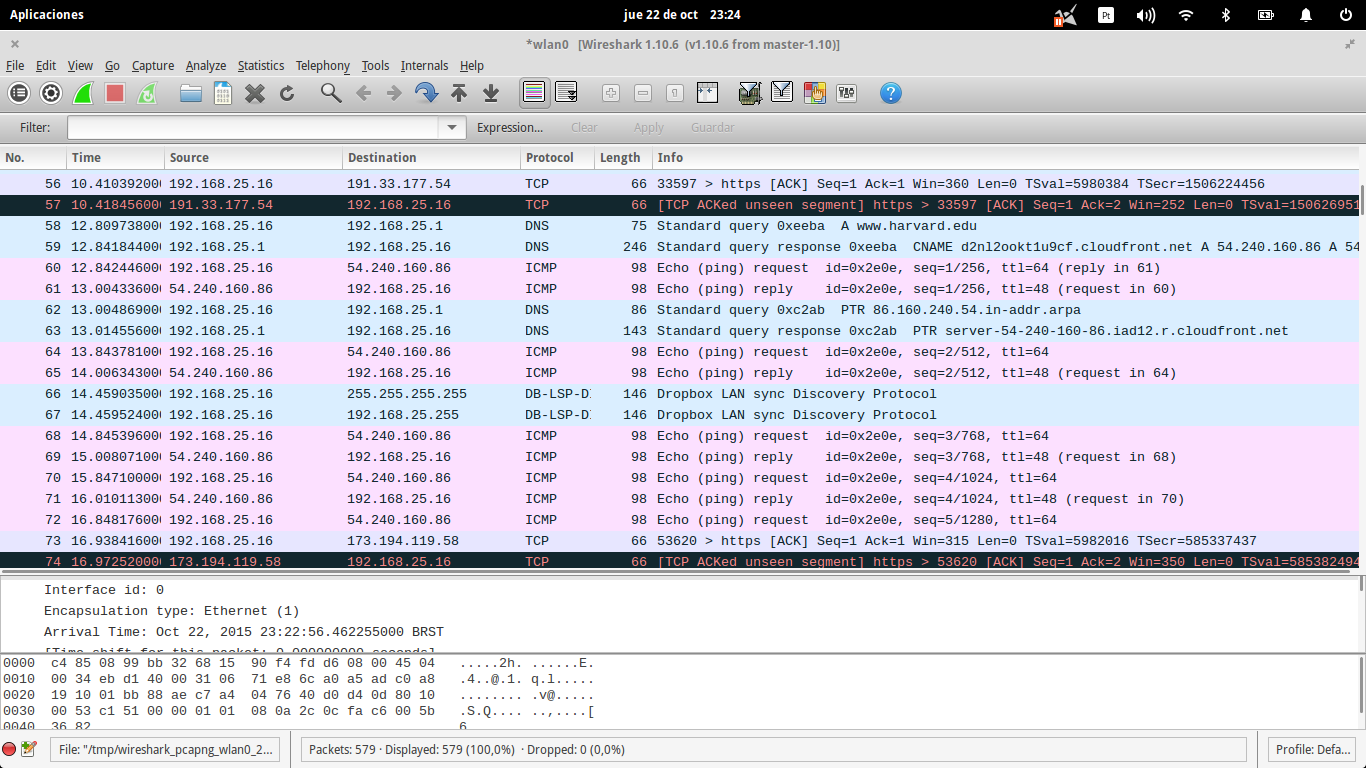
\includegraphics[width=450px, scale=1]{figuras/ping}
    \caption{Resultado do comando PING no terminal}

 \label{fig:1}
  \end{figure}

Observando ainda esta imagem, nota-se que o pacote percorreu 255-243 = 12 hosts até a chegada do destino (servidor do \emph{locaweb.com.br}). Além disso, ainda é possível observar pelas estatísticas que dos 5 pacotes de 64 bits enviados, todos os pacotes foram enviados e nenhum perdido e que o tempo médio foi 27,4 ms.

Já na imagem a seguir, é apresentado o print do resultado do analisador de pacote uma vez que o comando ping foi executado.

  \begin{figure}[h]
    \centering

    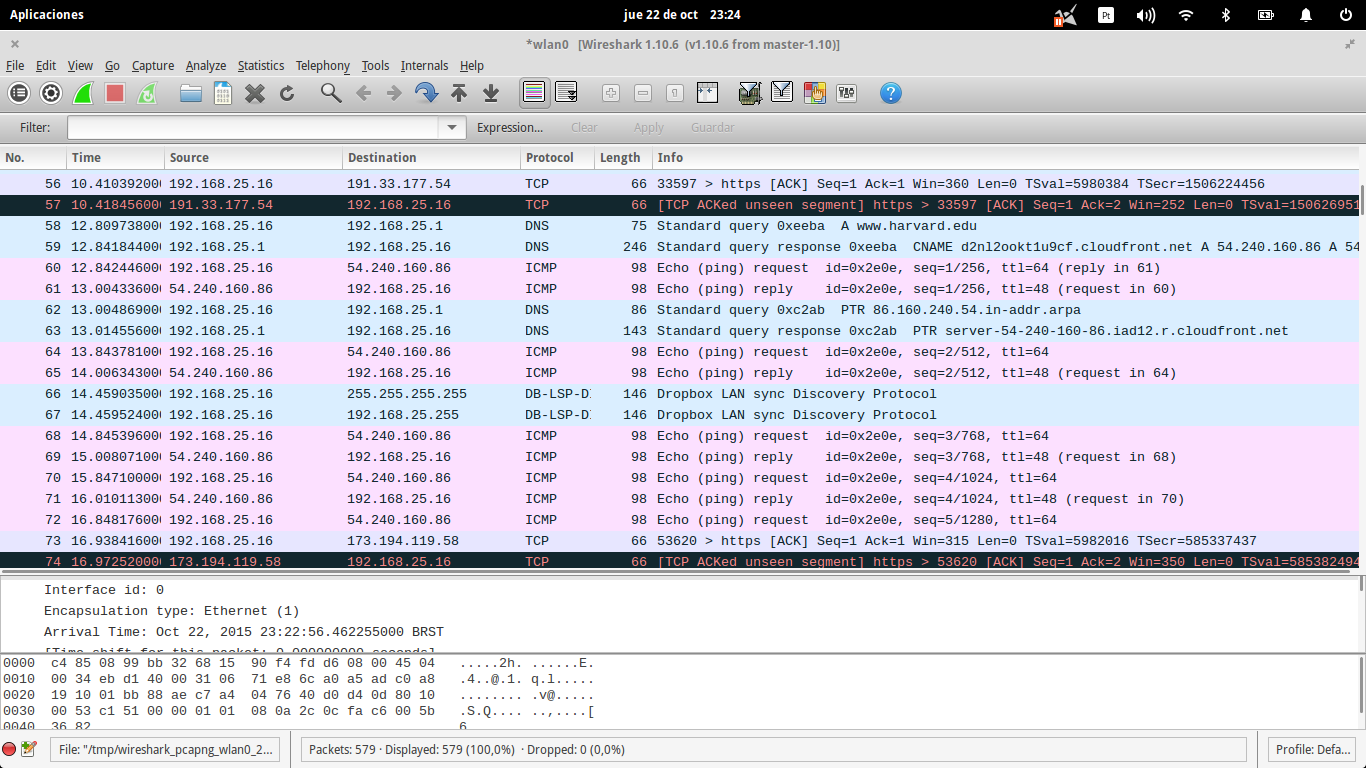
\includegraphics[width=450px, scale=1]{figuras/ping}
    \caption{Capturas de Pacotes em uma transação PING - Parte 1}

 \label{fig:2}
  \end{figure}

Como pode ser observado na imagem anterior, o PING enviar um pacote ICMP (da camada de redes) \emph{echo request} isto é, apenas uma requisição ao host, e aguarda uma mensagem \emph{echo reply}, isto é, uma resposta da requisição encaminhada.
	
Assim como dito anteriormente, o ping pode ser utilizado para verificar a conectividade entre dois hosts. Neste caso, está sendo estabelecida uma conexão entre o host solicitante (\emph{192.168.25.10}) e o host destino (\emph{186.202.147.77}). Inicialmente, o host solicitante encaminha uma echo request (type 8) para o destino. Como ilustra a imagem a seguir, o pacote capturado é um ICMP do tipo echo request.

  \begin{figure}[h]
    \centering

    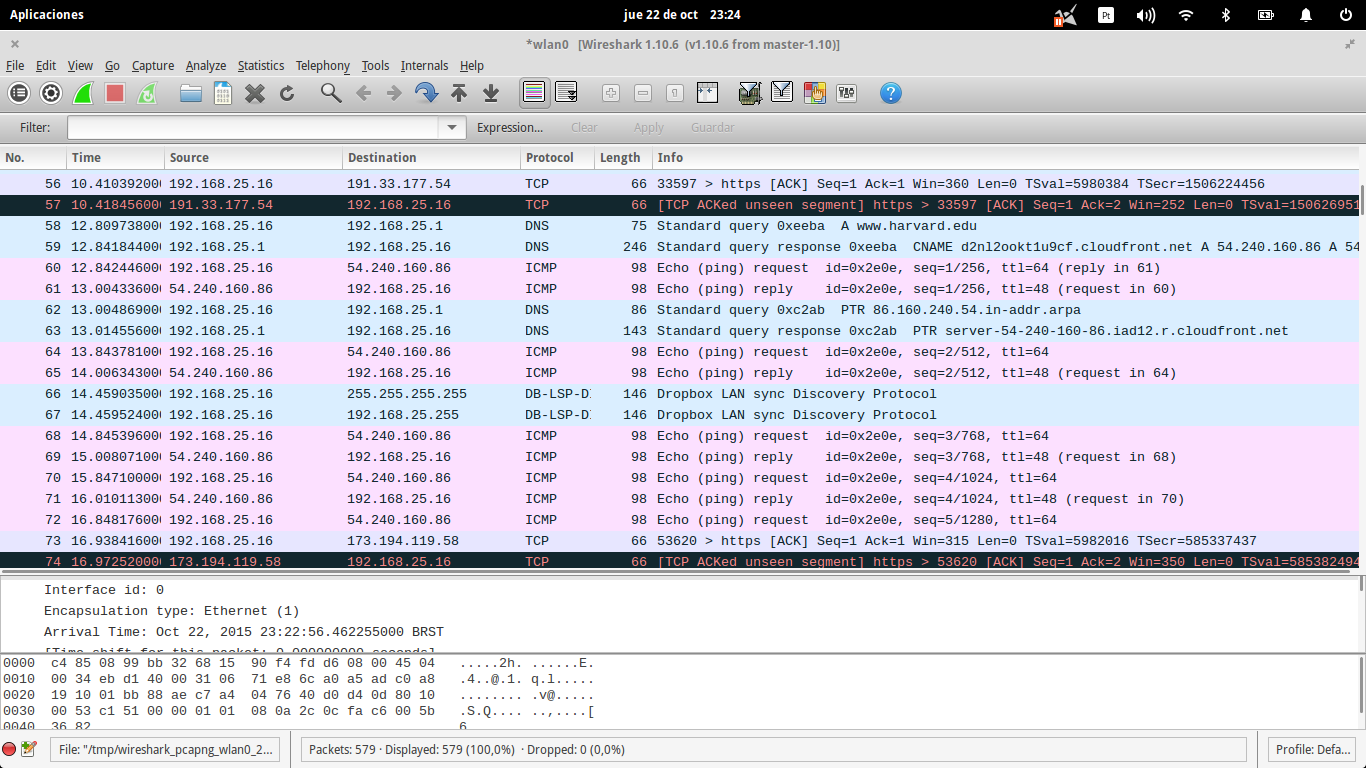
\includegraphics[width=450px, scale=1]{figuras/ping}
    \caption{Capturas de Pacotes em uma transação PING - Parte 1}

 \label{fig:2}
  \end{figure}

Em seguir, o destino manda um pacote do tipo \emph{echo reply} (type 0) respondendo a requisição. Como ilustra a imagem a seguir, o pacote capturado é um ICMP do tipo \emph{echo reply}.


  \begin{figure}[h]
    \centering

    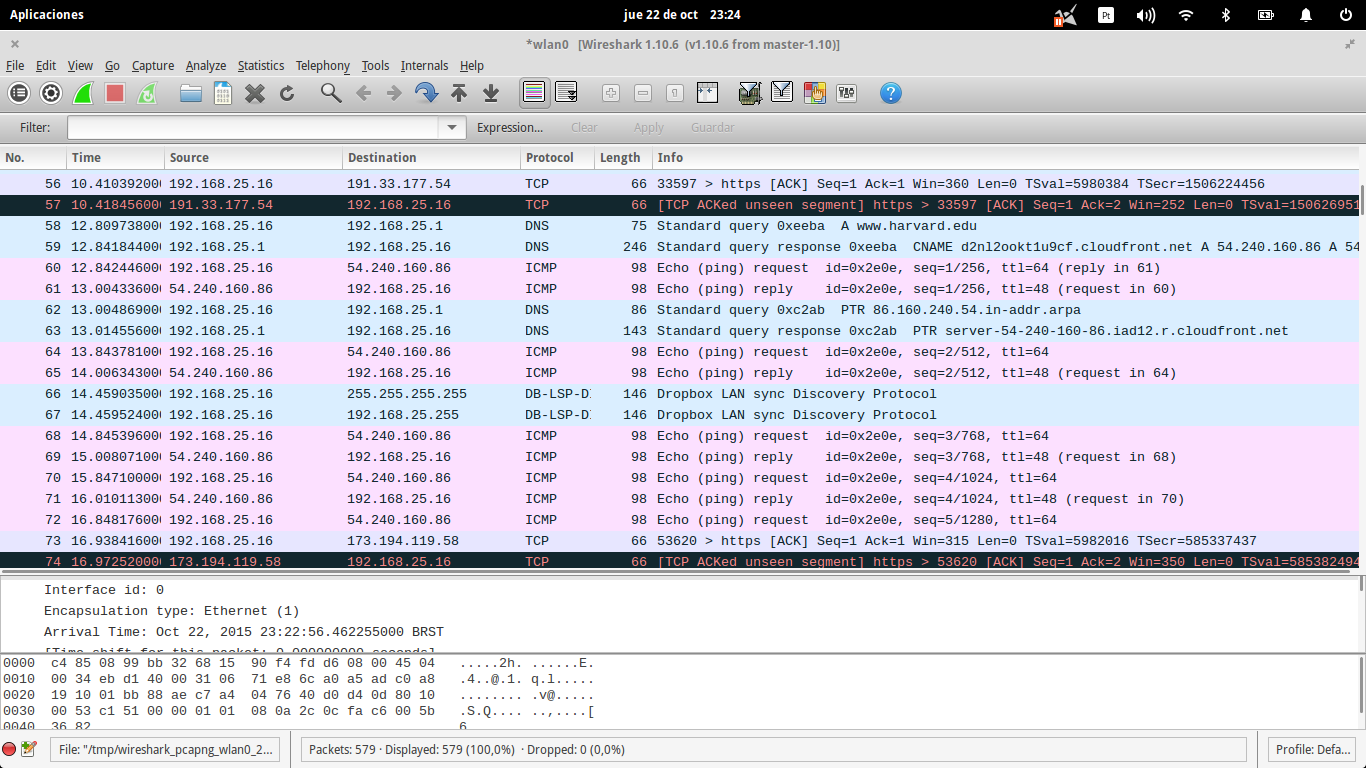
\includegraphics[width=450px, scale=1]{figuras/ping}
    \caption{Capturas de Pacotes em uma transação PING - Parte 2}

 \label{fig:3}
  \end{figure}

A partir dessas duas imagens, verifica-se que há uma perfeita conexão entre o host origem e o host destino. No entanto, há a possibilidade do pacote se perder e neste caso, é apresentada estáticas em relação a perde de pacotes, como mostra o exemplo na imagem a seguir, no qual foi feito um ping www.microsoft.com.

 \begin{figure}[h]
    \centering

    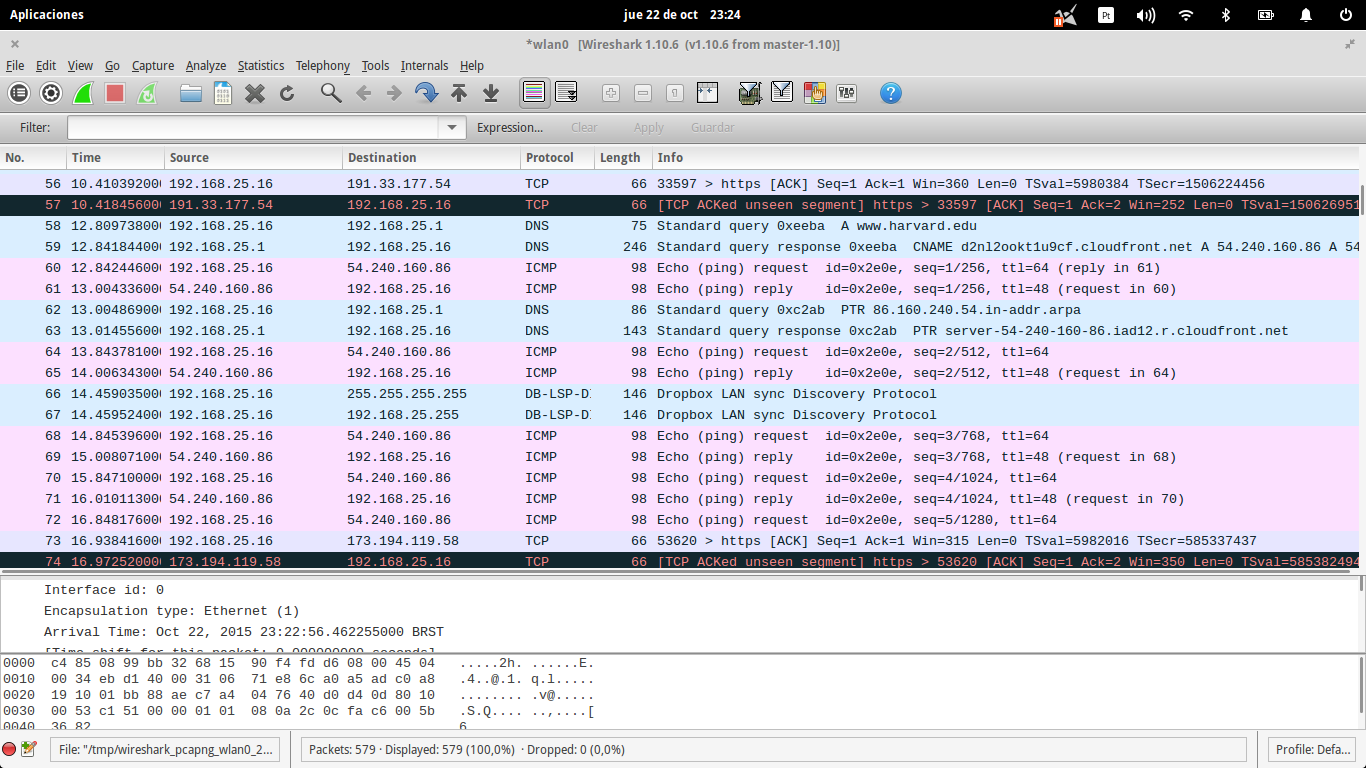
\includegraphics[width=450px, scale=1]{figuras/ping}
    \caption{Resultado do PING com pacote perdido}

 \label{fig:4}
  \end{figure}

Neste caso, percebe-se que um pacote foi perdido dos nove pacotes enviados. No entanto, mesmo com a perda do pacote, no qual pode ter sido ocasionada por exemplo pelo forçamento do final da execução do ping (\emph{ctrl + C}), houve uma conexão com o servidor solicitado.


\section{Mensagens Utilizando Nmap}

O \textbf{NMAP} é uma ferramenta útil para verificar rapidamente as portas abertas em determinado host, seja na sua rede local, seja na Internet.

Durante a utilização da ferramenta, foi verificado o uso do protocolo DNS da camada de aplicação para a resolução do endereço de host passado (google.com). Neste caso, foi utilizado o protocolo UDP para a camada de transporte e o protocolo IPv4 na camada de rede.

Uma vez resolvido o endereço de IP de destino para o host google.com(\emph{186.215.92.89}), os pacotes trocados entre o host de teste e o host de destino, utilizaram o TCP como protocolo de transporte e o IPv4 como protocolo de rede.

O processo típico de testes proporcionado pelo \textbf{NMAP} consiste na inicialização do analisador de pacotes, configurando­ para monitorar uma porta de rede do dispositivo utilizado para o teste. O \textbf{NMAP} recebe o host com o qual deverá se comunicar através de linha de comando nos sistemas Unix. Uma vez que a troca de pacotes entre o host local de teste e o host indicado pelo comando ocorre utilizando­-se a porta que está sendo monitorada, todos os pacotes trocados farão parte da lista de pacotes monitorados pelo analisador e pacotes.

O \textbf{NMAP} também é capaz de mostrar todas as portas que podem ser utilizadas para a comunicação com o host de destino e o tipo de serviço oferecido pela porta.

\begin{figure}[h]
    \centering

    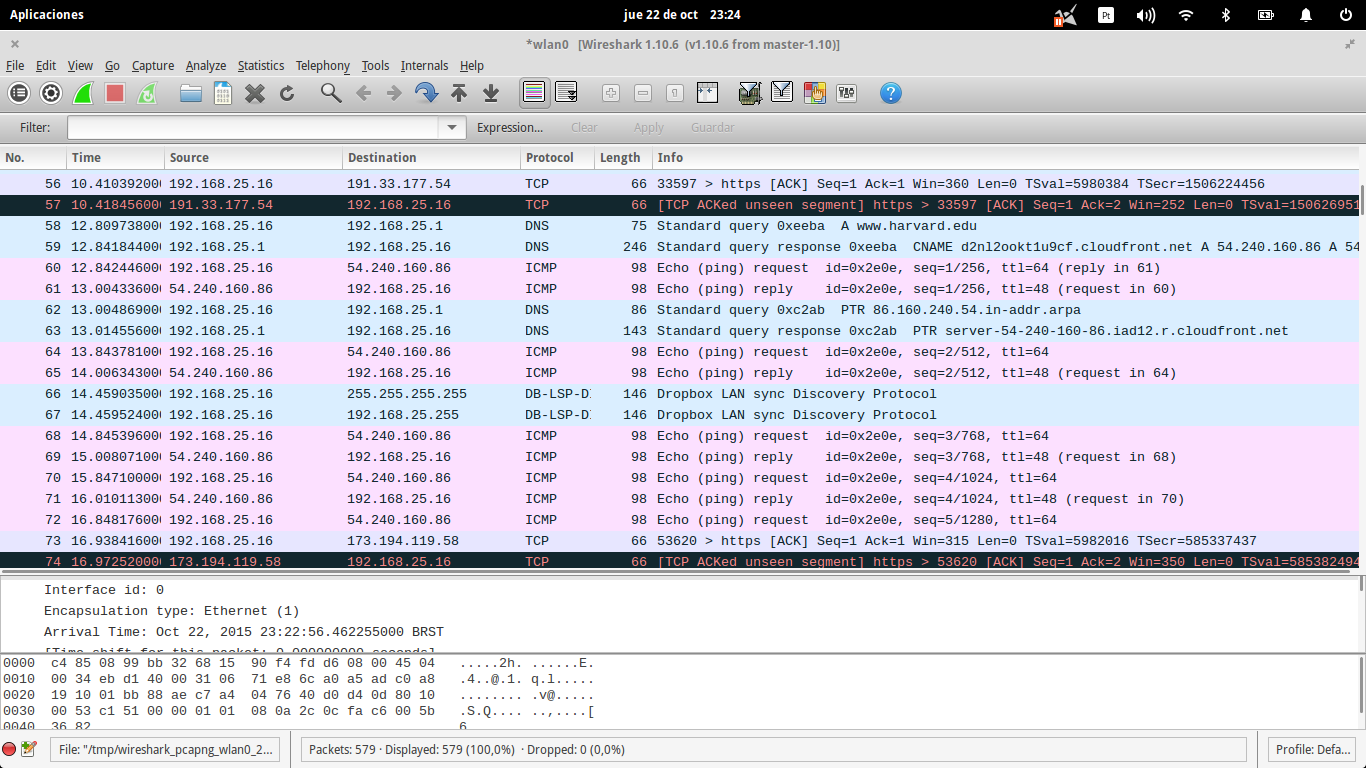
\includegraphics[width=450px, scale=1]{figuras/ping}
    \caption{Resultado do comando NMAP}

 \label{fig:nmap}
  \end{figure}

  Não foram detectados pacotes com problemas durante a execução de testes utilizando o \textbf{NMAP}.


\section{Mensagens Utilizando Traceroute}

O \textbf{Traceroute} é uma ferramenta útil para observar a trajetória de um pacote de dados até um determinado host, permitindo então a detecção de possíveis problemas de roteamento.

Assim como no teste do NMAP, foi utilizado na camada de aplicação o DNS para a resolução do endereço de host passado (google.com). Também foram identificados o uso do protocolo UDP e IPv4 para as camadas de transporte e rede, respectivamente.
O endereço de IP de destino para o host google.com encontrado no primeiro teste foi 186.215.92.123. Os pacotes mostrados no analisador de pacotes utilizado identificou o protocolo UDP como protocolo da camada de transporte e o IPv4 como protocolo da camada de rede.

O processo de testes utilizado pelo \textbf{Traceroute} se baseia na conexão entre roteadores do caminho entre o host de origem e o host de destino. O \textbf{Traceroute} faz a troca de pacotes entre os hosts afim de apontar quantos e quais serão os hops do caminho que um pacote deverá seguir para que ocorra a troca de pacotes entre os mesmos.

Foram identificados pacotes que apontavam problemas com o TTL, indicando que o mesmo era de valor baixo ou não experado.
